\documentclass[main.tex]{subfiles}

\begin{document}

\chapter{Fenomenologia interazioni deboli}

\section{Processi deboli}
\subsection{Non leptonic}
Barione \PSigmaplus: $\ket{\Pqu\Pqd\Pqs}$.~\ref{subsec:sigma}
Mesone \PKplus: $\ket{\APqu\Pqc}$.~\ref{subsec:kaon}

\begin{align*}
\PSigmaminus&\to\Pneutron+\Ppiminus\\
\PKplus&\to \Ppiplus+\Ppizero\\
&\to\Ppiplus+\Ppiminus+\Ppiplus
\end{align*}

\subsection{Semi-leptonic}
Charmed meson D: Vedi \nameref{mesonD}
\begin{align*}
\beta^-&:\, ^A_ZX_N\to ^A_{Z+1}X_{N-1}+\Pelectron+\APnue \quad (\Pneutron\to\Pproton+\Pelectron+\APnue)\\
\beta^+&:\,^A_ZX_N\to^A_{Z-1}X_{N+1}+\APelectron+\Pnue\quad (\Pproton\to\Pneutron+\APelectron+\Pnue)&\intertext{Ha Q negativo avviene solo in un nucleo}\\
\epsilon&:\,^A_ZX_N+\Pelectron\to^A_{Z-1}X_{N+1}+\Pnue \quad (\Pproton+\Pelectron\to\Pneutron+\Pnue)\\
&\PDzero\to\PKminus+\APmuon+\Pnum
\end{align*}

\subsection{Purely leptonic}
\begin{align*}
\Pmuon  \to  \Pelectron +\APnue +\Pnum\\
L_e:\quad 0=1-1+0\\
L_{\mu}:\quad 1=0+0+1
\end{align*}

\section{Dove nel chart di Segre}

\begin{figure}[!ht]
\centering
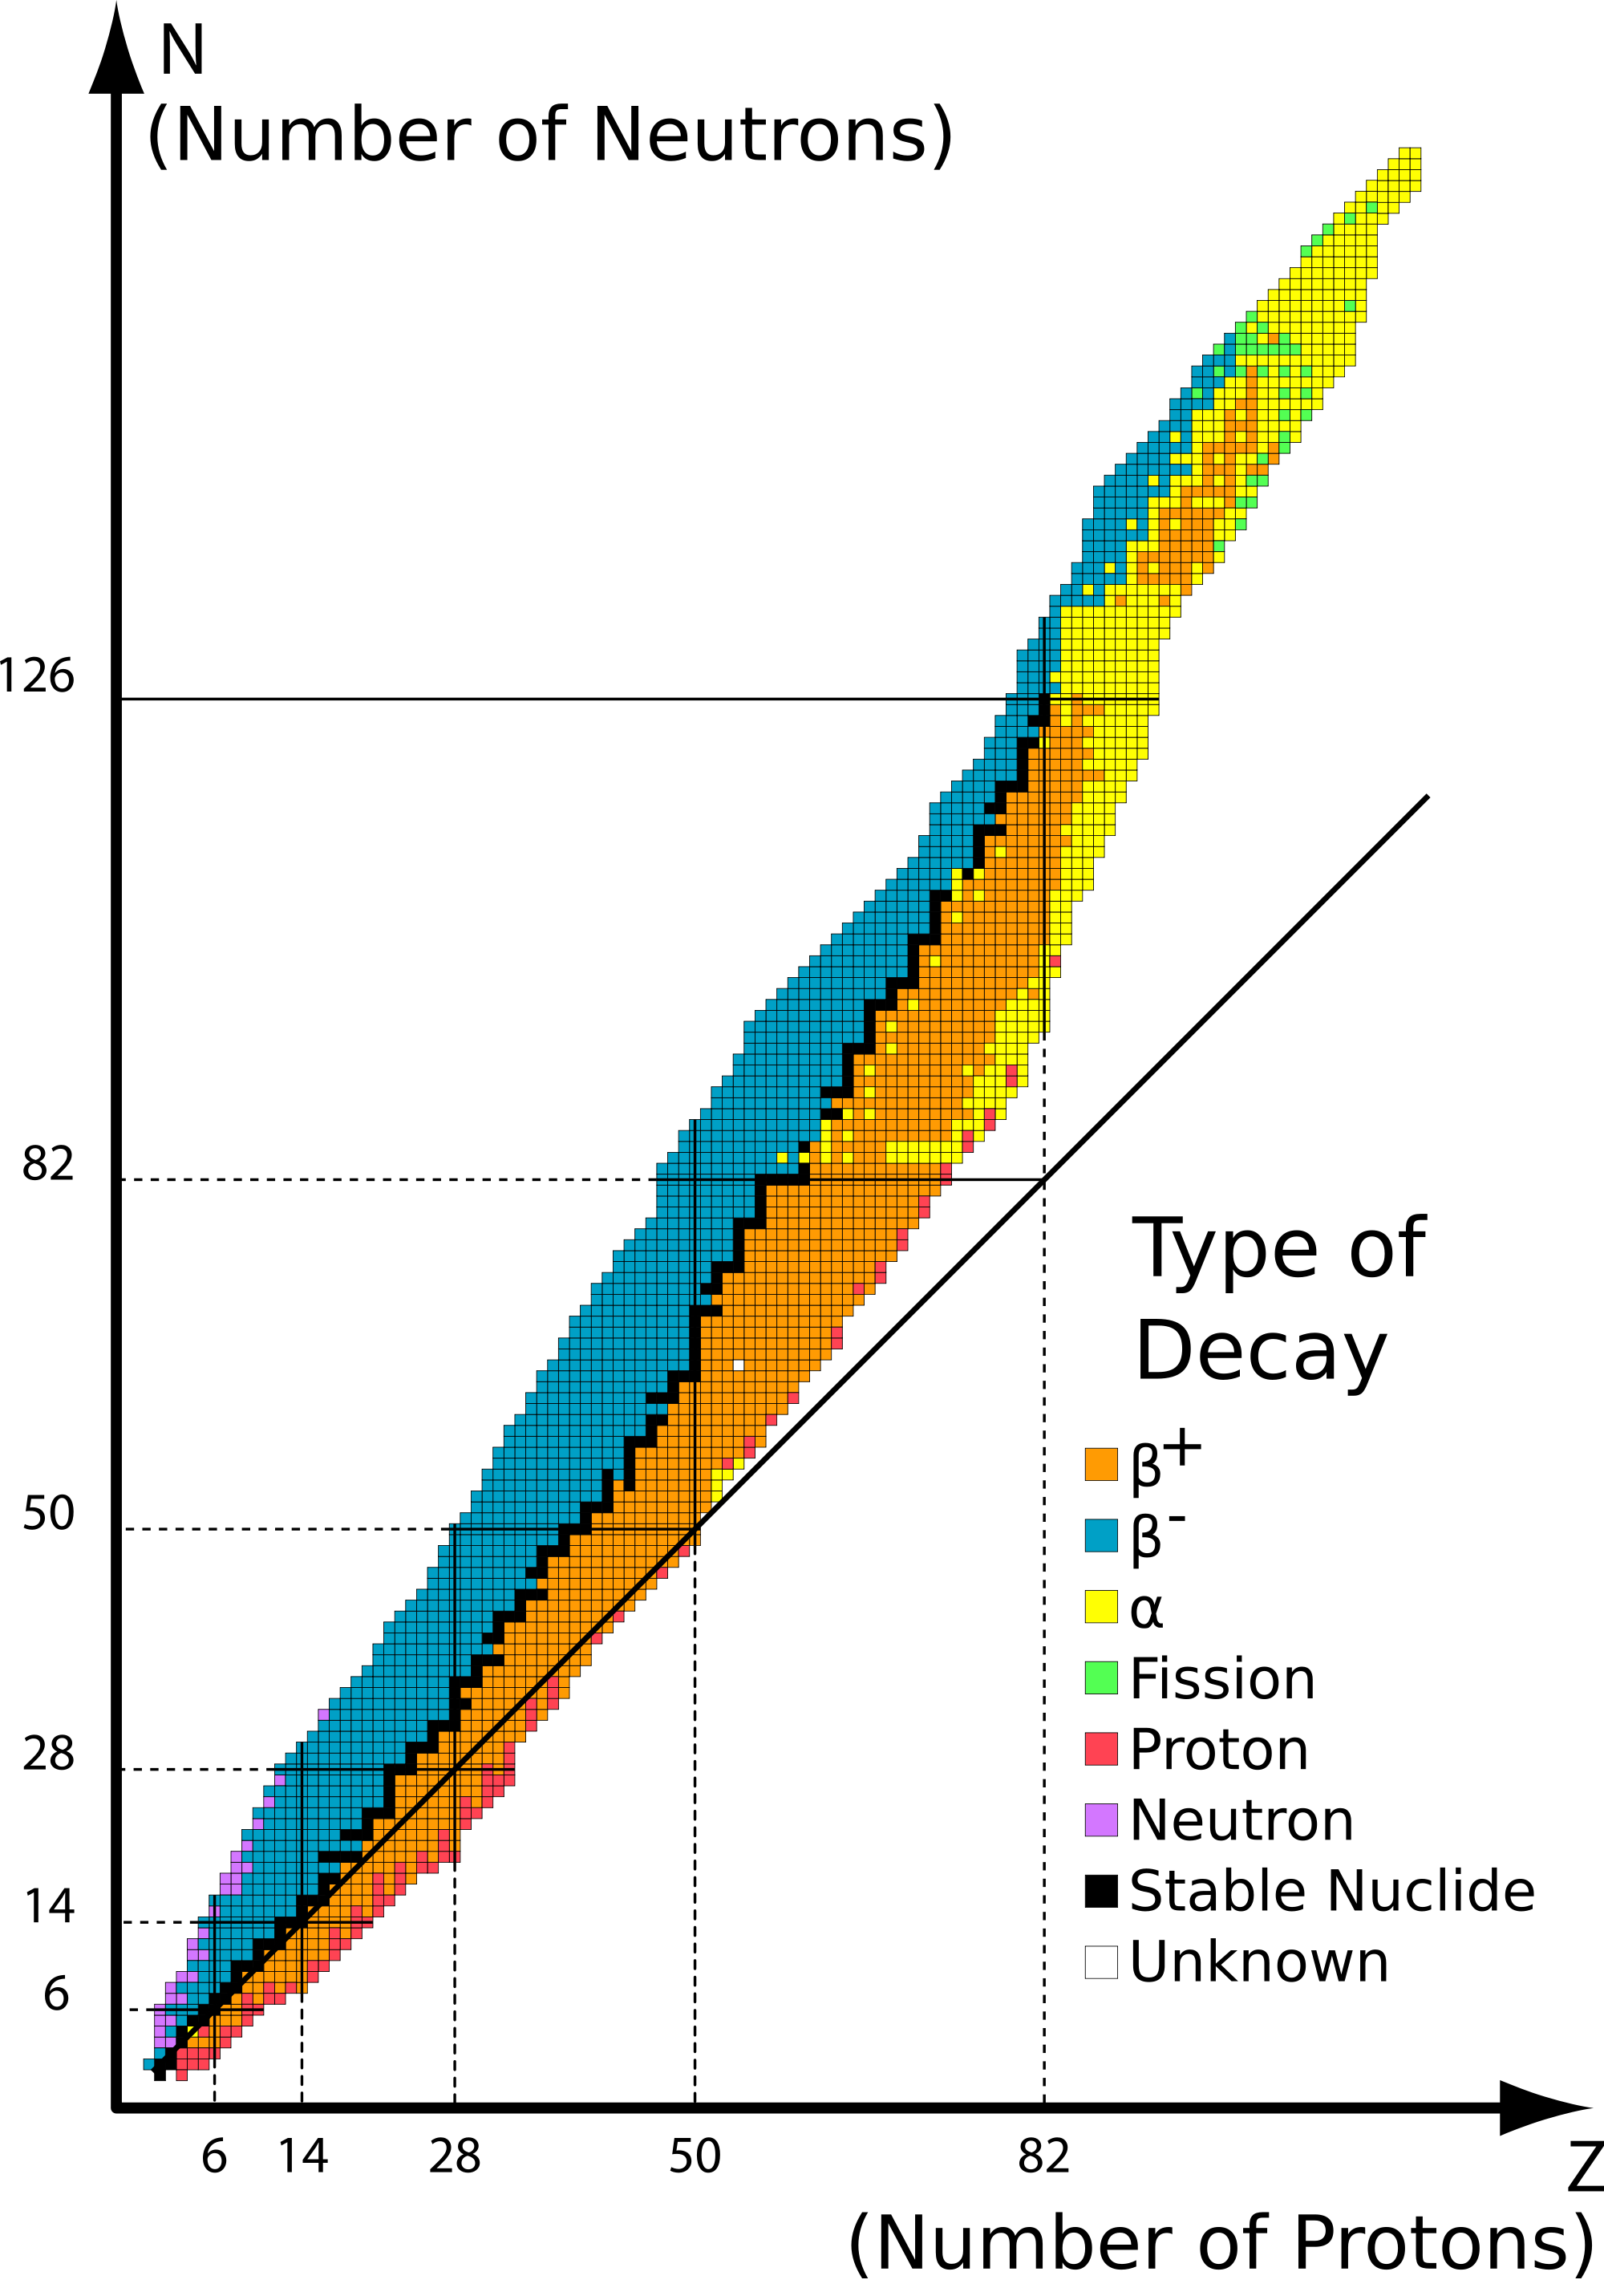
\includegraphics[width=\textwidth,height=(\textheight-21mm),keepaspectratio]{decayzones}
\caption{Zone Chart segre beta processes}
\label{fig:betaSegrec}
\end{figure}

\section{Parabola di massa}

\subsection{Formula semiempirica}
\begin{align*}
&M(A,Z)=Zm_P+(A-Z)m_N-B(A,Z)\\
&B(A,Z)=a_VA -a_SA^{\frac{2}{3}}-a_C\frac{Z(Z-1)}{A^{\frac{1}{3}}}-a_{Sym}\frac{(A-2Z)^2}{A}\\
&+\Delta(A,Z)&\intertext{l'ultimo termine comporta una differenza tra nuclei con A dispari e con A pari}
\end{align*}

La parabola \'e centrata nel nucleo isobaro pi\'u stabile (di massa minore)

\begin{align*}
\frac{\partial M}{\partial Z}&=0\\
Z_{min}&=\frac{\overbrace{[m_N-m(^1H)]}^{=m_N-m_P+B_e}+\overbrace{a_CA^{-\frac{1}{2}}}^{< 1 MeV}+4a_{Sym}}{2a_CA^{-\frac{1}{3}}+8a_{Sym}A^{-1}}&\intertext{i primi 2 termini del numeratore sono trascurabile, essendo:}\\
a_C&=0.72 MeV\quad a_{Sym}=23 MeV\\
&\approx\frac{A}{2}\frac{1}{1+\frac{1}{4}A^{\frac{2}{3}}a_C/a_{sym}}
\end{align*}
 Per nuclei pesanti $\frac{Z}{A}\approx0.41$.

\subsection{Configurazione pi\'u stabile ad A costante}
\begin{figure}[!ht]
\centering
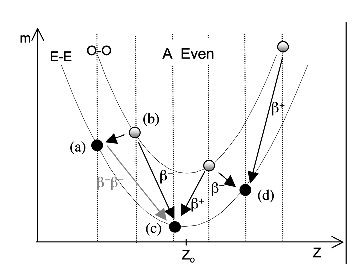
\includegraphics[width=(\linewidth-30mm),keepaspectratio]{parabola}
\caption{Parabola di massa}
\label{fig:parmas}
\end{figure}

\subsection{Esempi di decadimenti}
\begin{align*}
\bm\quad^{23}Ne\to^{23}Na+\Pelectron+\APnue\\(Q=4.38 MeV)\,(\thalf=38 s)\\
\bm\quad^{99}_{43}Tc\to^{99}_{44}Ru+\Pelectron+\APnue\\(Q=0.29 MeV)\,(\thalf=2.1*10^5 yr)\\
\bp\quad^{25}_{13}Al\to^{25}_{12}Mg+\APelectron+\Pnue\\(Q=3.26 MeV)\,(\thalf=7.2 s)\\
\bp\quad^{124}_{53}I\to^{124}_{52}Te+\APelectron+\Pnue\\(Q=2.14 MeV)\,(\thalf=4.2 d)\\
\ec\quad^{15}_{8}O+\Pelectron\to^{15}_{7}N+\Pnue\\(Q=2.75 MeV)\,(\thalf=1.2 s)\\
\ec\quad^{41}_{20}Ca+\Pelectron\to^{41}_{19}K+\Pnue\\(Q=0.43 MeV)\,(\thalf=1.0*10^5 yr)\\
\end{align*}

\section{A three body decay}

\subsection{Spettro energetico}
Nel 1919 Chadwick distinse lo spettro mono-energetico dell'electron capture e lo spettro continuo del decadimento beta.

Nel caso dello spettro continuo si pose il problema della conservazione dell'energia:
\begin{enumerate*}
\item Punto finale dello spettro corrisponde all'energia disponibile dalla disintegrazione (Q)
\item Indagini calorimetriche non rivelarono emissione di energia diversa da quella della particella beta
\end{enumerate*}

E anche della conservazione del momento angolare:
\begin{align*}
^3H\to^3He+\Pelectron\\
\frac{1}{2}\neq 0,1+l&\intertext{0,1 sono i possibili valori per gli accoppiamenti degli spin dei prodotti}
\end{align*}

\subsection{Neutrino}
Pauli nei primi anni trenta ipotizza l'esistenza di una particella neutra (conservazione della carica) e spin semi-intero (conservazione momento angolare) e massa a riposso quasi nulla che spieghi lo spettro continuo con $T_e^{max}\approx Q$.

Definizione
\begin{align*}
\Pproton\to\Pneutron+\Pelectron+\Pnue\\
\Pneutron\to\Pproton+\APelectron+\APnue
\end{align*}
Lo spin del neutrino \'e antiparallelo al momento, lo spin dell'anti-neutrino \'e parallelo al momento.

\begin{equation*}
^{38}Cl(2^-)\to^{38}Ar(0^+)+\Pelectron(\frac{1}{2}^+)+\APnue(\frac{1}{2}^-)
\end{equation*}

L'elicit\'a del neutrino \'e il coseno dell'angolo tra lo spin e la direzione del moto: per particelle con massa a riposo nulla \'e ''conservata''.

The chirality/handedness operator does not commute with the hamiltonian unless if the mass is zero. Hence, although we don't know yet the physical observable which is associated with this operator we do know that it is conserved and corresponds to a good quantum number only if the mass is zero or can be neglected.

So far we considered chirality/handedness for massless fermions. However, the ''chirality properties`` of massive fermions are also of interest. The reason for this is that most particles are massive and the charged current weak interaction couples to left handed (negative chirality) spinors (V-A theory).

As seen here the left handed positive energy spinor has contributions from both positive and negative helicity components. However the negative helicity component is dominant and becomes $100\%$ in the case where the mass is much smaller than the energy and can be neglected. The positive helicity component decreases $\propto\frac{M}{E}$	and approaches zero as the energy increases.

\subsection{Q-valore}

\begin{itemize*}
\item $\bm$:

\begin{align*}
&^A_ZX_N\to^A_{Z+1}X_{N-1}+\Pelectron+\APnue\\
Q&=[m(Z,A)-m(Z+1,A)-m_e]c^2\\
&=M(^A_ZX_N) -M(^A_{Z+1}X_{N-1})\\
&-Zm_e+(Z+1)m_e-m_e+\overbrace{\sum^ZB^i_e-\sum^{Z+1}B^i_e}^{\approx eV}&\intertext{con buona approssimazione il Q-valore del beta meno}\\
Q&=[M(^A_ZX_N)-M(^A_{Z+1}X_{N-1})]c^2
\end{align*}

\item $\bp$:

\begin{align*}
&^A_ZX_N\to^A_{Z-1}X_{N+1}+\APelectron+\Pnue\\
Q&=m(A,Z)-m(A,Z-1)\\
&=M(^A_ZX_N)-Zm_e-M(^A_{Z-1}X_{N+1})\\
&+(Z-1)m_e-m_e[\sum^ZB_e^i-\sum^{Z-1}B_e^i]\\
&\approx [M(^A_ZX_N)-M(^A_{Z-1}X_{N+1})-2m_e]c^2
\end{align*}

\item $\ec$:

\begin{align*}
&^A_ZX_N+\Pelectron\to^A_{Z-1}X_{N+1}+\Pnue\\
Q&=m(A,Z)+m_e-m(A,Z-1)\\
&=M(A,Z)-Zm_e+m_e-M(^A_{Z-1}X_{N+1})\\
&+(Z-1)m_e-\sum^{Z-1}B_e^i+\sum^ZB_e^i\\
&=M(A,Z)-M(A,Z-1)+B_e^n&\intertext{l'ultimo termine \'e la binding energy dell'elettrone catturato}
\end{align*}
\end{itemize*}

La cattura di un elettrone interno \'e seguita da emissione a cascata di radiazione EM dovuta alle transizioni elettroniche: l'energia emessa \'e pari alla BE dell'elettrone catturato?

\chapter{Teoria di Fermi}
Introducendo un nuovo parametro spiega
\begin{enumerate*}
\item Forma spettri beta
\item Relazione tra vita media e massima energia degli elettroni
\item Classificazione transizioni beta e regole di selezione
\end{enumerate*}

\section{Probabilit\'a di transizione: regola d'oro.}


\begin{equation*}
w=\frac{2\pi}{\hbar}|H_{if}|^2\rho(E_f)
\end{equation*}

\subsection{Densit\'a di stati finali.}

La densit\'a di stati finali determina completamente la forma dellop spettro beta:

Chiamo 
\begin{equation*}
\rho(E_f)=\frac{dn}{dE_F}
\end{equation*}
il numero di stati con energia in $[E_F,E_F+dE_F]$.

\subsection{Elementi di matrice}
\begin{align*}
H_{if}=\int\psi_f^*H\psi_id^3x&\intertext{ho indicato le funzioni d'onda degli stati iniziali e finali}\\
\ket{\psi_i}=\ket{u_i}\quad\ket{\psi_f}=\ket{u_f}\ket{\phi_e}\ket{\phi_{\nu}}
\end{align*}

\subsection{Interazione debole come perturbazione.}
Uno stato stazionario ha energia definita:
\begin{equation*}
\Delta t*\Delta E\geq\frac{\hbar}{2}\quad\Rightarrow\quad\Delta t=\infty,\,\Delta E=0
\end{equation*}
Aggiungendo una piccola perturbazione all'Hamiltoniana $V'$ posso avere transizioni tra autostati di H imperturbata.
\begin{equation*}
\Delta E=\Gamma\neq0,\quad\tau=\frac{\hbar}{\Gamma}
\end{equation*}
Probabilit\'a di decadimento
\begin{align*}
\lambda=\frac{1}{\tau}=\frac{2\pi}{\hbar}|V_{fi}|^2\rho(E_f)&\intertext{l'ultimo membro esprime la regola d'oro fi Fermi}
\end{align*}

\section{Approssimazione transizioni permesse.}

\subsection{Hamiltoniana debole: ipotesi di Fermi.}
\begin{align*}
&H_{if}=g\int\psi_f^*O_XH\psi_id^3x&\intertext{X pu\'o indicare Vector, Axial-scalar, Scalar, Pseudo-scalar, Tensor}\\
&\bm:\quad O_X\propto T_+\\
&\bp:\quad O_X\propto T_-\quad\bp
\end{align*}

\subsection{Approssimazione interazione di contatto}
\begin{align*}
&r_{int}=\frac{\hbar c}{m_Wc^2}=\frac{200 MeV*fm}{8*10^4 MeV}=2.5*10^{-3}\approx0
&V_{Weak}=gO_X\delta^3(\vec{r_e}-\vec{r_i})\delta^3(\vec{r_{\nu}}-\vec{r_i})
\end{align*}

\subsection{Probabilit\'a di transizione: transizioni permesse.}
Funzioni d'anda elettrone e neutrino: approssimazione onde piane.
\begin{align*}
&\phi_e(\vec{r})=\frac{1}{\sqrt{V}}\exp{i\scap{k_e}{r}}\\
&\phi_{\nu}(\vec{r})=\braket{\vec{r}|\phi_{\nu}}=\frac{1}{\sqrt{V}}\exp{i\scap{k_{\nu}}{r}}
\end{align*}

quindi

\begin{align*}
&\braket{\psi_f|V_{deb}|\psi_i}=\\
&\frac{1}{V}g\int\exp{-i\scap{r_e}{r_i}}\exp{-i\scap{r_{\nu}}{r_i}}\psi_f^*(\vec{r_1},\ldots,\vec{r_i},\ldots,\vec{r_A})O_X\psi_i(\vec{r_1},\ldots,\vec{r_i},\ldots,\vec{r_A})
\end{align*}

Approssimazione transizioni permesse.

\begin{align*}
\exp{i\scap{k_e}{r_i}}&\approx1\\
\exp{i\scap{k_{\nu}}{r_i}}&\approx1\intertext{\Pelectron e \APnue vengono emessi in onda S. In generale vale l'espansione}\\
\exp{i\scap{k}{r}}&=\sumzi{l}i^l(2l+1)j_l(kr)P_l(\cos{\theta})\abc{kr\approx0}1+i\scap{k}{r}\ldots
\end{align*}

Giustifico
\begin{align*}
&E_e=T_e+mc^2=\sqrt{(p_ec)^2+(m_ec^2)^2}\\
&T_e\approx1 MeV\Rightarrow P_ec=\sqrt{T_e^2+2m_ec^2T_e}\approx1.42 Mev\\
&k_e=\frac{p_e}{\hbar}=\frac{p_ec}{\hbar c}\approx7*10^{-3}fm^{-1}\\
&\scap{k_e}{r_i}\leq k_eR\leq10^{-2}&\intertext{R \'e il raggio del nucleo}
\end{align*}

risulta
\begin{equation*}
\braket{\psi_f|V_{weak}|\psi_i}=\frac{g}{V}\overbrace{\braket{\psi_f|O_X|\psi_i}}^{M_{if}}\\
w=\frac{1}{\tau}=\frac{2\pi}{\hbar}\frac{g^2}{V^2}|M_{fi}|^2\rho(E_f)
\end{equation*}

Considerazioni
\begin{itemize*}
\item Le funzioni d'onda devono essere trattate da spinori di Dirac
\item $H_{if}$ deve descrivere anche l'emissione di \APelectron con l'aggiunta del termine c.h. ad H
\item Add terms with different parity selection rule
 \end{itemize*}

\section{Momentum and kinetic energy spectra}

\subsection{Chiarimento notazioni}

Definisco alcune quantit\'a adimensionalin (Segre)
\begin{align*}
&E_e=\epsilon mc^2\\
&p_e=\eta mc\\
&Q=\epsilon_0mc^2\\
&p_e^{max}=\eta_0 mc
\end{align*}

Segre usa $W=E_{\nu}+E_e$ Krane usa $Q=W-m_ec^2$.

\subsection{Fattori che compongono lo spettro beta}

\begin{align*}
\frac{dN}{N}\frac{1}{dt}=\lambda=\frac{2\pi}{\hbar}|M_{if}|^2\rho{E_f}
\end{align*}

Lo spettro beta contiene 3 fattori:

\begin{enumerate*}
\item $p_e^2(Q-T_e)^2$ derived from the number of final states available to emitter.
\item La funzione di Fermi $F(Z,\epsilon)$: correzione per il campo Coulombiano del nucleo.\index{Funzione di Fermi}

Espressione approssimata.
\begin{align*}
&F(Z,\epsilon)=\frac{2\pi n}{1-\exp{-2\pi n}}\\
&n=\pm\frac{Ze^2}{\hbar v_e}\\
&n\approx0\quad\Rightarrow\quad F(Z,\epsilon)\approx1
\end{align*}

\item Se $M_{fi}=0$ in approx. transizione permessa devo considerare il termine successivo dell'espansione dell'onda piana. Ne tengo conto co un termine $S(p_e,p_{\nu})$.
\end{enumerate*}
Lo spettro in funzione del momento dell'elettrone
\begin{equation*}
N(p)\propto p^2(Q-T_e)^2F(Z',p)|M_{fi}|^2S(p,q)
\end{equation*}

\subsection{Densit\'a di stati finali}

Calcolo numero stati in $[k,k+\,dk]$
\begin{align*}
dn_e=\frac{V4\pi p_e^2\,dp_e}{h^3}=\frac{V4\pi k_e^2\,dk_e}{(2\pi)^3}\\
dn_{\nu}=\frac{V4\pi p_{\nu}^2\,dp_{\nu}}{h^3}=\frac{V4\pi k_{\nu}^2\,dk_{\nu}}{(2\pi)^3}
\end{align*}

Lo spin \'e un grado di libert\'a?

L'elicit\'a dell'elettrone nel decadimento beta \'e negativa, del positrone \'e positiva, del \APnue positiva e del \Pnue negativa.

Densit\'a di stati finali con energia in $[Q,Q+\,dQ]$ e momento dell'elettrone in $[p_e,p_e+\,dp_e]$
\begin{align*}
\frac{dn}{dE_F}\frac{dn}{dQ}&=dn_e\frac{dn_{\nu}}{dQ}\\
&=\frac{V^2}{h^6}(4\pi)^2p_e^2(\frac{Q-T_e}{c})^2\frac{1}{c}dp_e
&\intertext{ho eliminato la dipendenza dal momento del neutrino, di cui trascuro la massa, tramite}\\
Q-E_e=E_{\nu}=cp_{\nu}
\end{align*}

\subsection{Probabilit\'a di decadimento parziale}


La probabilit\'a di decadimento con elettrone finale in $[p_e,p_e+\,dp_e]$
\begin{equation*}
w(p_e)\,dp_e=\frac{2\pi}{\hbar c}g^2|M_{if}|^2\frac{(4\pi)^2}{(2\pi\hbar)^6}\frac{(Q-E_e)^2}{c^2}p_e^2dp_e
\end{equation*}


\subsection{Total decay rate}
Costante di decadimento totale (indipendente dal momento dei prodotti)
\begin{align*}
\lambda&=\int_0^{p_e^{EP}}w(p_e)dp_e\\
&=\frac{g^2|M_{fi}|^2}{2\pi^3c^3\hbar^7}\int_0^{P_e^{Max}}[Q-\sqrt{m^2c^4+c^2p_e^4}]^2p_e^2\,dp_e
\end{align*}

\subsection{Shape of beta spectrum}

Nella sezione sopra ho trovato lo spettro in funzione del momento

\begin{align*}
&N(p)\propto\frac{1}{c^2}p^2(Q-T_e)^2\\
&\propto\frac{1}{c^2}p^2(Q-\sqrt{(pc)^2+(m_ec^2)^2}+m_ec^2)^2&\intertext{La costante \'e $C=\frac{V^2(4\pi)^2}{(2\pi\hbar)^6}$.}
\end{align*}

e trovo quello in energia

\begin{align*}
&N(T_e)=\frac{C}{c^5}\sqrt{T_e+2T_em_ec^2}(Q-T_e)^2(T_e+m_ec^2)&\intertext{ricavato considerando che}\\
&T_e+mc^2=\sqrt{(p_ec)^2+(m_ec^2)^2}\\
&\Rightarrow\, c^2p\,dp=(T_e+m_ec^2)\,dT_e
\end{align*}

Spettro elettronico con energia in $[T_e,T_e+\,dT_e]$.

\begin{figure}
\centering
\subfloat{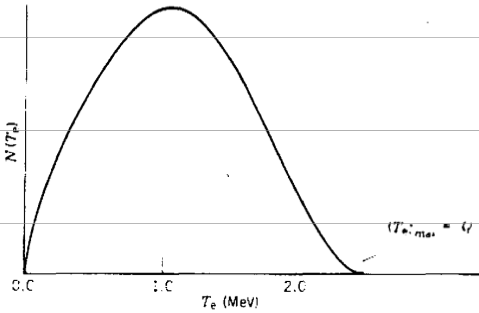
\includegraphics[width=(\textwidth-10pt)/2,height=(\textheight-11mm),keepaspectratio]{betaEspectrum}}\,
\subfloat{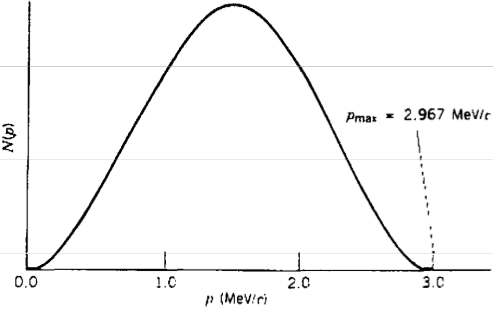
\includegraphics[width=\textwidth,height=(0.2\textheight),keepaspectratio]{betapspectrum}}
\caption{Spettro in funzione di p ed E della radiazione beta}
\end{figure}

\clearpage

\section{Vita media comparativa. Plot Furmi-Kurie.}

\subsection{Integrale di Fermi.}

\begin{align*}
&f(Z',E_0)=\frac{1}{(m_ec)^3(m_ec^2)^2}*\\
&*\int_0^{p_{max}}F(Z',p)p^2(E_0-\sqrt{(cp_e)^2+(m_ec^2)^2})\,dp_e\\
&cp_e^{max}=\sqrt{E_0^2-(m_ec^2)^2}&\intertext{$\uparrow$ maximum total electron energy}\\
&=\int_0^{P_e^{EP}}F(Z',E_e)(\frac{p_e}{m_ec})^2(\frac{E_0-E_e}{m_ec^2})\frac{\,dp_e}{m_ec}\\
\midrule\\
&\lambda=\frac{g^2m^5c^4}{2\pi^3\hbar^7}|\Mif|^2f(\eta_0)\\
&f(\eta_0)=\int_0^{\eta_0}[\sqrt{1+\eta_0^2}-\sqrt{1+\eta^2}]^2\eta^2\,d\eta&\intertext{quest'ultimo \'e l'integrale di Fermi in variabile adim. con $F(Z',E_e)=1$}
\end{align*}

\subsection{Plot Fermi-Kurie.}

Parto dallo spettro del momento elettronico in funzione di var. adim.
\begin{align*}
&w(\eta),d\eta=\frac{g^2m^5c^4}{2\pi\hbar^7}|M_{fi}|^2[\sqrt{1+\eta_0^2}-\sqrt{1+\eta^2}]^2\eta^2\,d\eta&\intertext{per transizioni permesse e tenendo conto della funzione di Fermi F il plot (di Kurie)}\\
&\sqrt{\frac{w(\eta)}{\eta^2F(Z',\epsilon)}}\quad vs\quad(\epsilon-\epsilon_0)&\intertext{\'e una retta, cio\'e: essendo}\\
&(Q-T_e)\propto\sqrt{\frac{N(p)}{p^2F(Z',p)}}&\intertext{graficando il secondo membro vs energia cinetica \Pelectron ho una retta che intercetta x in Q.}
\end{align*}

\begin{figure}
\centering
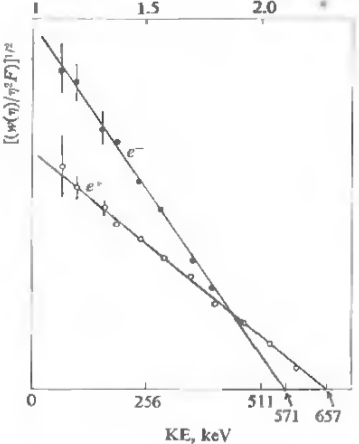
\includegraphics[width=(0.7\textwidth),height=(\textheight),keepaspectratio]{fermikurieplot}
\caption{Kurie plot of the $^{64}Cu$ beta spectra}
\end{figure}

\clearpage

\subsection{Massa del neutrino.}

Ricavo la relazione $p_{\nu}(T_e)$ nel caso di $m_{\nu}\neq0/m_{\nu}=0$.

\begin{align*}
&m_{\nu}=0:\quad Q=T_e+p_{\nu}c\,\Rightarrow\, p_{\nu}=\frac{1}{c}(Q-T_e)\\
&N_e(p_e)\propto p_e^2p_{\nu}^2\frac{dp_{\nu}}{dE_f}=\\
&p_e^2(Q-T_e)^2\quad\lim_{p_e\to p_e^{Max}}{\frac{dN_e(p_e)}{dp_e}}=0&\intertext{$\uparrow$ per $m_{\nu}=0$}\\
&m_{\nu}\neq0:\quad Q=T_e+\frac{p_{\nu}^2}{2m_{\nu}}\,\Rightarrow\, p_{\nu}=\sqrt{2m_{\nu}}\sqrt{Q-T_e}\\
&p_e^2\sqrt{Q-T_e}\quad\lim_{p_e\to p_e^{Max}}{\frac{dN_e(p_e)}{dp_e}}=-\infty&\intertext{$\uparrow$ per $m_{\nu}\neq0$}
\end{align*}

Sperimentalmente:

\begin{equation*}
T\to^3He+\Pelectron+\APnue,\quad \thalf=12.3 yr,\quad Q=18.6KeV
\end{equation*}

This is a good choice since
\begin{itemize*}
\item low Q-value make the influence of small neutrino mass stand more prominent in Kurie plot
\item $^3He$ has high excited states so the ground state is the result of decay
\end{itemize*}

\begin{figure}
\centering
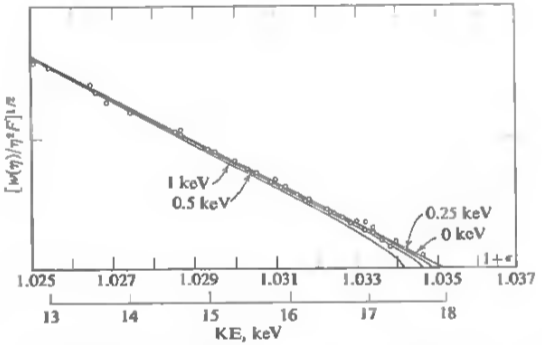
\includegraphics[width=(0.9\textwidth),height=(\textheight),keepaspectratio]{neutrinomassFKplot}
\caption{Upper end of a Fermi plot for $^3H$ compared with curves for different neutrino rest energy.}
\end{figure}

\clearpage

\subsection{Vita media comparativa.}

Confronto processo beta in nuclei diversi:
\begin{align*}
&\lambda=\frac{m_e^5c^4}{2\pi^3\hbar^7}g^2|\Mif|^2f(Z',E_0)=\frac{1}{\tau}=\frac{\ln{2}}{\thalf}\\
&f*\thalf=0.693\frac{2\pi^3\hbar^7}{g^2m_e^5c^4|\Mif|^2}
\end{align*}

differenze di $ft$ son dovute a alementi di matrice differenti quindi differenti funzioni d'onda nucleari.

$ft$ varia in un grande intervallo di valori: sperimentalmente si ha che piccoli valori di $ft$ cio\'e elevati elementi di matrice si hanno solo se $\Delta I=\pm1,0$.

\subsection{Superallowed decays: strenght of weak interaction}
The decays with shortest $ft$ ($\log{ft}\approx3-4$) are known as superallowed decay.

\begin{align*}
\lambda&=\frac{m_e^5c^4}{2\pi^3\hbar^7}g^2|\Mif|^2f(Z',E_0)\\
&=\frac{G^2}{2\pi^3}\frac{mc^2}{\hbar}|\Mif|^2f(Z',\epsilon_0)
\end{align*}

Per superallowed $0^+\to0^+$ decay calcolo $|\Mif|=\sqrt{2}$:
\begin{align*}
f*\thalf=0.693\frac{2\pi^3\hbar^7}{g^2m_e^5c^4|\Mif|^2}&\intertext{posso ricavare g dalla misura di $ft$}\\
g=0.88*10^{-4}\,MeV\,fm^3
\end{align*}

In forma adimensionale: introduco una massa arbitraria $\mathcal{M}$
\begin{equation*}
G=\frac{g}{\mathcal{M}^{-2}\hbar^3c^{-1}}=g\frac{\mathcal{M}^2c}{\hbar^3}
\end{equation*}

Per interazioni NN \'e logico usare $m_p$:
\begin{align*}
G(m_p)=G_{Weak}=10^{-5}&\intertext{per interazione forte ho }\\
G(m_{\Ppi})=1
\end{align*}

\chapter{V-A theory}

\section{Teorema di Wigner-Eckart}

\subsection{Vettori in QM}

\begin{equation*}
[V_i,J_j]=i\epsilon_{ijk}\hbar V_k
\end{equation*}

\subsection{Tensori sferici}

Definizione (CR).

\begin{align*}
&[J_z,T_q^{(k)}]=\hbar qT_q^{(k)}\\
&[J_{\pm},T_q^{(k)}]=\hbar\sqrt{(k\mp q)(k\pm q+1)}T_{q\pm1}^{(k)}
\end{align*}

\subsection{m-selection rules}

\begin{equation*}
\braket{\alpha',j'm'|T_q^{(k)}|\alpha,jm}\neq0 \Leftrightarrow m'=q+m
\end{equation*}

\subsection{T. di Wigner-Eckart}

\begin{align*}
&\braket{\alpha',j'm'|T_q^{(k)}|\alpha,jm}=\braket{jk;mq|jk;j'm'}\frac{\braket{\alpha'j'||T^{(k)}||\alpha j}}{\sqrt{2j+1}}&\intertext{il primo fattore \'e il CCG per la somma di j e k a j'.}
\end{align*}

Le regole di selezione per gli elementi di matrice del tensore sono le stesse della somma di momenti angolari.

\subsection{Esempi: rank $k=0,1$.}

\begin{align*}
&\braket{\alpha',j'm'|S|\alpha,jm}\propto\delta_{mm'}\delta_{jj'}\\
&\vec{V}\to V_{q=\pm1,0}^{(1)}:\quad\Delta m=m'-m=\pm1,0\quad\Delta j=\pm1,0
\end{align*}

\subsection{Teorema di proiezione}

\begin{align*}
\braket{\alpha',jm'|T_q^{(k)}|\alpha,jm}=\frac{\braket{\alpha',jm|\scap{J}{V}|\alpha,jm}}{\hbar^2j(j+1)}\braket{jm'|J_q|jm}
\end{align*}

\subsection{Esercizio: Momento di quadrupolo}

\begin{enumerate*}

\item Scrivi $xy,\ xz,\ (x^2-y^2)$ come componenti di un tensore sferico irriducibile di rango 2.

\item Momento di quadrupolo

\begin{align*}
Q=e\braket{\alpha jm=j|(3z^2-r^2)|\alpha jm=j}\\
e\braket{\alpha jm'|(x^2-y^2)|\alpha jm=j}&\intertext{valutare questa espressione $\uparrow$ in termini di Q e dei CCG appropriati.}
\end{align*}

\end{enumerate*}

 \subsection{Esercizio: Interazione momento quadrupolo nucleare/external inhomogeneous electric field}

\section{Nuclear transiction matrix element: allowed transiction, Fermi decay, Gamow-Teller decay.}

\subsection{Nuclear part of beta decay operator}
Dato che un \Pneutron \'e trasformato in un \Pproton dal decadimento $\bm$ e al contrario da $\bp$ l'operatore che causa il decadimento deve coinvolgere un nucleone alla volta, cio\'e i singoli operatori di salita e discesa per l'isospin dei nucleoni.

\begin{align*}
O_{\lambda,\mu}(\beta)=G_V\sum_{J=1}^A\vec{\tau_{\mp}}(J)+G_A\sum_{J=1}^A\vec{\sigma}(J)\vec{\tau}(J)&\intertext{The first term carries angular momentum $\lambda=0$ the second $\lambda=1$}
\end{align*}

According to the V-A theory, there are two terms in the weak interaction, a polar vector part with coupling constant $G_V$ and an axial-vector part with coupling constant $G_A$ . In the nonrelativistic limit, the vector  part may be represented by the unity operator times $\tau_{\mp}$ and the axial-vector part by a product of the intrinsic spin operator $\vec{\sigma}$ and $\tau_{\mp}$.

\subsection{Long wavelength approx.: allowed transition}

\begin{align*}
\ket{\phi_0(\vec{r})}=\ket{J_iM_i\zeta}\\
\ket{\phi_{\vec{k}}(\vec{r})}=\frac{1}{\sqrt{V}}\exp{i\scap{k_e}{r}}\frac{1}{\sqrt{V}}\exp{i\scap{k_{\nu}}{r}}\ket{J_fM_f\xi}
\end{align*}

Considero le funzioni d'onda dei leptoni
\begin{align*}
\exp{\scap{k}{r}}=\sumzi{\lambda}\sqrt{4\pi(2\lambda+1)}i^{\lambda}j_{\lambda}(kr)Y_{\lambda 0}(\theta,0)&\intertext{dove ho definito}\\
k=|\vec{k}|=|\vec{k_e}+\vec{k_{\nu}}|\quad\theta=\angle{\vec{k_e},\vec{k_{\nu}}}
\end{align*}

In the long wavelenght approx $kr\ll1$:
\begin{equation*}
j_{\lambda}(kr)\approx\frac{(kr)^{\lambda}}{(2\lambda+1)!!}
\end{equation*}

Considerando solo i termini $\lambda=0$ e $\lambda=1$
\begin{equation*}
\ket{\phi_{\vec{k}}(\vec{r})}=\frac{1}{V}[1+\sqrt{\frac{4\pi}{3}}(kr)Y_{10}(\theta,0)]\ket{J_fM_f\xi}
\end{equation*}
Transizioni dovute a termini pi\'u elevati sono inibiti nel beta-decay ancor di pi\'u che nel decadimento EM.

\subsection{Elemento di matrice di transizione. Approssimazione di transizioni permesse; Fermi and Gamow-Teller decay types.}

\begin{align*}
\braket{\phi_{\vec{k}}(\vec{r})|H'|\phi_0(\vec{r})}&\approx\frac{G_V}{V}\sum_{\mu M_f}[\\
&\braket{J_fM_f\xi|\sum_{J=1}^A\vec{\tau_{\mp}}(J)|J_iM_i\zeta}\\
&+\underbrace{g_A}_{=\frac{G_A}{G_V}}\braket{J_fM_f\xi|\sum_{J=1}^A\vec{\sigma}(J)\vec{\tau_{\mp}}(J)|J_iM_i\zeta}]&\intertext{Il primo braket tra parentesi rappresenta un decadimento di Fermi il secondo di Gamow-Teller}
\end{align*}

L'approssimazione di transizioni permesse consiste nel considerare solo i 2 termini di ordine pi\'u elevato.

\subsection{Conserved vector current hypothesis}
\begin{align*}
\Pproton\leftrightarrow\Ppiplus+\Pneutron&\intertext{Electric charge is unchanged, magnetic interaction changed}\\
\end{align*}
In beta decay $g_F$ is unchanged by surrounding meson's cloud (like electric charge) while $g_{GT}$ may be affected (like magnetic moment).

\section{Allowed approx: regole di selezione.}

\subsection{Fermi type decay: matrix element}

Considero \Pelectron, \APnue creati in $r=0$:

sono emessi da una particella puntiforme ($\frac{R}{\lambda(\Plepton)}\ll1$) quindi non trasportano momento e il cambiamento dello momento angolare del nucleo \'e dovuto agli spin dei \Plepton (Composizione di 2 spin $\frac{1}{2}$: $S=0,1$). Gli spin del \Pelectron e del \APnue sono antiparalleli: stato antisimmetrico di singoletto, $S=0$.



Nel caso delle transizioni di Fermi posso sommare gli operatori di salita/discesa sui nucleoni per formare quello di salita/discesa dell'isospin del nucleo
\begin{equation*}
\sum^A\tau_{\mp}(J)=T_{\mp}
\end{equation*}

L'elemento di matrice pu\'o essere calcolato senza conoscere le funzioni d'onda nucleari
\begin{align*}
&\braket{J_fM_fT_fT_{0f}|\sum\tau_{\mp}|J_iM_iT_iT_{0i}}\\
&=\sqrt{T_i(T_i+1)-T_{0i}(T_{0i}\mp1)}\delta_{J_fJ_i}\delta_{M_fM_i}\delta_{T_fT_i}\delta_{T_{0f,T_{0i}\mp1}}
\end{align*}

L'interazione Coulombiana e $m(\Ppipm)\neq m(\Ppizero)$ violate isospin symmetry and affect actual value of Fermi matrix element.

\subsection{Fermi type decay: selection rules}
\begin{align*}
&J_f=J_i\\
&T_f=T_i\neq0 (\Delta T=0; T_i=0\to0=T_f \text{Forbidden})&\intertext{F operator has isospin rank 1}\\
&T_{0f}=T_{0i}\mp1 (\Delta T_0=1)\\
&\Delta\Pi=0
\end{align*}

\subsection{Gamow-Teller type decay: selection rules}
Gli spin dei \Plepton sono paralleli: $S=1$.

Spherical tensor rank are unity in spin and isospin spaces.
\begin{align*}
&\Delta J=0,1 (J_i=0\to0=J_f\quad\text{forbidden})\\
&\Delta T=0,1 (T_i=0\to0=T_f\quad\text{forbidden})\\
&T_{0f}=T_{0i}\mp1 (\Delta T_0=1)\\
&\Delta\Pi=0&\intertext{$\vec{\sigma}$ is axial vector}
\end{align*}

\subsection{Superallowed decay}

\begin{equation*}
J_i^{\Pi_i}=0^+\to0^+=J_f^{\Pi_f},\quad\Delta\Pi=0
\end{equation*}

\begin{itemize*}
\item Decadimento $\bm$ \'e spesso inibito dal Q-valore negativo: energia Coulombiana maggiore per il nucleo finale.
\item GT term do not contribute
\item Least sensitivity to details of nuclear wave function
\item Measure $G_V$: light nuclei.
\item Positron emitter.

\begin{align*}
&^{14}O\to^{14}N+\APelectron+\Pnue\quad\thalf=74s,\,Q=1.12 MeV&\intertext{il prodotto \'e nel primo eccitato $0^+$ con}\\
&E^{ex}=2.311 MeV
\end{align*}

\end{itemize*}

\subsection{Vita media comparativa}

\begin{align*}
\sum|\braket{i|O_{\lambda\mu}|f}|^2=G_V^2[\exv{F}^2+g_A^2\exv{GT}^2]
\end{align*}
Per le transizioni permesse
\begin{align*}
ft=\frac{K}{\exv{F}^2+g_A^2\exv{GT}^2}\\
K=\frac{2\pi^3\hbar^7\ln{2}}{m_e^5c^4G_V^2}=6141 s&\intertext{da K ricavo }\\
\frac{G_V}{(\hbar c)^3}=1.149*10^{-11}MeV^{-2}
\end{align*}

\section{Forbidden decay}

\subsection{Regole di selezione}
Abbiamo $\Delta J>1$: fattore $ft$ maggiore e quindi minore probabilit\'a di decadimento.
Il fattore centrifugo per $l>0$ inibisce l'emissione di leptoni:

in 1-MeV decay if electron is given all energy $p=1.4 MeV/c$ quindi con il raggio nucleare $R\approx6 fm$ ho $\frac{pR}{\hbar}\approx0.04<1$ so the most frequent occurrence is when $\Pi_i\neq\Pi_f$.

\begin{equation*}
\Delta J=l,\,l\pm1,\quad\Delta\Pi=(-1)^l
\end{equation*}

\subsection{Definite spherical tensor rank}
\begin{enumerate*}
\item First order forbidden operators.
\begin{equation*}
rY_{1\mu}(\theta,\phi)\propto\vec{r},\quad(\vec{\sigma}\wedge Y_1(\theta,\phi))_{\lambda=0,1,2\,\mu}
\end{equation*}
% ancora pg 36 e wong 210
\end{enumerate*}

\section{Parit\'a}

%segrepg338
%QuestionofParityConservationinWeakInteractions

\subsection{Particelle $\tau-\theta$}
Nel 1956 si sono imbattuti in 2 particelle ($\tau-\theta$) che hanno stessa vita media,stesso spin e stessa massa ma decadono in sistemi di pioni di parit\'a opposta.
Se la parit\'a si conserva sono particelle diverse: Lee e Yang misero in dubbio la conservazione della parit\'a nelle interazioni deboli.

\subsection{Solenoide riflesso}
Considero l'emissione di elettroni di un nucleo di cobalto in spira percorsa da corrente: il campo magnetico orienta spin nucleare in modo che la corrente del solenoide e la corrente del nucleo siano parallele. Fissiamo che lo spin e il campo magnetico sono lungo z: sperimentalmente risulta che gli elettroni vanno di preferenza nella direzione negativa delle z (a sinistra). Il sistema ottenuto riflettendo quello di partenza su uno specchio parallelo all'asse del solenoide non da un sistema reale: invertendo la corrente del solenoide il massimo dell'intensit\'a della radiazione beta \'e a destra.

\subsection{Vettori polari e assiali}
Vettori polari sono detti quelli che per inversione di coordinate rispetto all'origine si invertono.
\begin{equation*}
\vec{p}\,\vec{x}
\end{equation*}

Vettori assiali sono detti quelli che per inversione di coordinate rispetto all'origine restano immutati.
\begin{equation*}
\vec{L},\quad\vec{S},\quad\vec{H},\quad\vec{\mu},\quad\vecp{r}{F}
\end{equation*}

Il prodotto tra un vettore polare e uno assiale cambia segno per inversione delle coordinate: lo chiamo pseudoscalare.

\subsection{Parity conserving + non conserving interaction}
Se l'immagine e l'oggetto debbono essere indistinguibili tutti gli pseudo scalari debbono annullarsi.

Se la parit\'a non \'e esattamente conservata dall'interazione che lega un sistema i suoi stati sono un mix di termini con parit\'a opposta.

Se indico con $F$ l'intensit\'a della forza che non conseva la parit\'a $F^2$ rappresenta il peso statistico degli stati che non conservano P: l'accuratezza delle regole di selezione di P per le transizioni atomiche e nucleari permette di stimare $F^2\leq(\frac{r}{\lambda})^2\approx10^{-6}$.

\subsection{Decadimento beta del cobalto polarizzato}
Nel 1956 Wu e altri effettuarono un esperimento volto a misurare lo pseudo-scalare 
\begin{equation*}
\exv{\scap{v}{I}}
\end{equation*}
Usarono $^{60}Co$ con spin polarizzato da campo magnetico lungo z: trovarono che la direzione di emissione di \Pelectron nel beta-decay a $^{60}Ni$ \'e di preferenza opposta alla direzione dello spin.

\chapter{Esempi}

\section{F decays}
\subsection{$0^+\to0^+$}
\begin{align*}
^{14}O\to^{14}N^*\\
^{34}Cl\to^{34}S\\
^{10}C\to^{10}B\\
\end{align*}

\subsection{$\frac{1}{2}^+\to\frac{1}{2}^+$}
\begin{align*}
\Pneutron\to\Pproton
\end{align*}
\section{GT decays}

\subsection{Pure GT}
\begin{align*}
^6He\to^6Li\quad(0^+\to1^+)\\
^{13}B\to^{13}C\quad(\frac{3}{2}^-\to\frac{1}{2}^-)\\
^{230}Pa\to^{230}Th^*\quad(2^-\to3^-)
\end{align*}

\subsection{Mixed F and GT decays}
\begin{align*}
^{111}Sn\to^{111}In\quad(\frac{7}{2}^+\to\frac{9}{2}^+)
\end{align*}

Chiamo $y=\frac{g_FM_F}{g_{GT}M_{GT}}$ e ancora
\begin{align*}
g^2|\Mif|^2&=g_F^2|\Mif^F|^2+g_{GT}^2|\Mif^{GT}|^2\\
&=g_F^2|\Mif^F|^2(1+y^{-2})
\end{align*}

\section{Neutron decay}

\begin{align*}
&\lambda=\frac{0.693}{\thalf}\propto G_F^2M_F^2(1+y^{-2})\\
&|M_F|=1
\end{align*}
Sperimentalmente ricavo $y=0.46\pm0.003$ cio\'e il decadimento \'e $82\%$ GT e $18\%$ F.

\section{Mirror decays}
\begin{align*}
^{41}_{21}Sc_{20}\to^{40}_{20}Ca_{21}
\end{align*}
Nel caso dei mirror decays il calcolo di $M_F$ e $M_{GT}$ \'e pi\'u facile: except for minor differneces due to Coulomb interaction the wave function of initial and final nucleus are the same.
$g_F$ and $M_F$ have the same values as they do for decay of free neutron.

%vedi tabelle pg 35

\part{Rivelazione neutrini}


\chapter{Correnti cariche/Correnti neutre}

\section{Weak interaction: exchange-force model}

\subsection{Intermediate vector boson}

\begin{figure}[!ht]
\centering
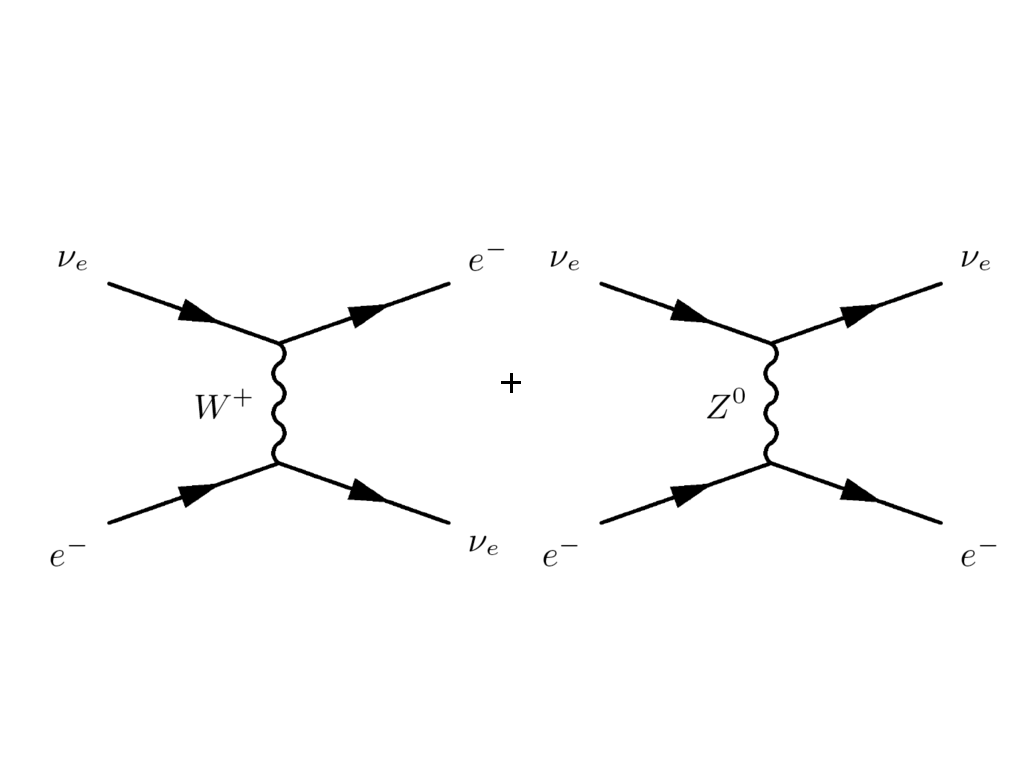
\includegraphics[width=(\linewidth-30mm)]{WpZ0}
\caption{Scambio e scattering mediato da W e Z.}
\end{figure}

\begin{itemize*}
\item \PWpm.

Mass $81GeV/c^2$.

Decay $\PWpm\to\Pepm+\Pnu$.

\item \PZzero.

Mass $93GeV/c^2$.

Decay $\PZzero\to\Pelectron+\APelectron$.

\end{itemize*}

\chapter{Tecniche di rivelazione}

\section{Scattering Compton}

Scattering Compton \'e il processo di scatter di un \Pphoton da parte di un \Pelectron quasi-legato ($B_e\ll E_{\Pphoton}$)

\subsection{Compton scattering formula}

\begin{equation*}
E_{\Pphoton}'=\frac{E_{\Pphoton}}{1+(\frac{E_{\Pphoton}}{mc^2})(1-\cos{\theta})}
\end{equation*}

\subsection{Klein-Nishina formula}

La probabilit\'a di scattering Compton ad angolo $\theta$ si calcola quantisticamente
\begin{align*}
&\frac{d\sigma_c}{d\Omega}=r_0[\frac{1}{1+\alpha(1-\cos{\theta})}]^3*[\frac{1+\cos{\theta}}{2}]\\
&[1+\frac{\alpha^2(1-\cos{\theta})^2}{(1+\cos{\theta}^2)[1+\alpha(1-\cos{\theta})]}]\\
&\alpha=\frac{E_{\Pphoton}}{mc^2}\\
&r_0=\frac{e^2}{(4\pi\epsilon_0)mc^2}\approx2.8 fm
\end{align*}

\section{Radiazione Cerenkov}

L'eletrone scatterato viaggia ad una velocit\'a superiore a quella della luce nel mezzo ($c'=\frac{c}{n}$): viene sfruttata l'emissione Cherencov concentrata in uno angolo solido ristretto (ring-like pattern) per ricavare l'energia della particella e la posizione iniziale.  

\section{Spettro dei neutrini solari}

La probabilit\'a delle diverse catene varia a seconda delle condizioni della stella quindi un modo per determinare le condizioni del core del sole \'e misurare lo spettro energetico dei neiutrini emessi e quindi la probabilit\'a relativa dei diversi processi.


\subsection{PP chain: neutrino mean energy}

\begin{tabular}{c|cc|}
\hline
Reaction & Q(MeV) & $\exv{q_{n_e}}$  \\
 \hline
$^1H(\Pproton,\APelectron\Pnue)^2H$ & $1.442$ & $0.265$\\
$^1H(\Pproton\Pelectron,\Pnue)H$ & $1.442$ & $1.442$\\ 
$^7Be(\Pelectron,\Pnue)^7Li$ & $0.862$ & $0.862$\\ 
$^8B(\APelectron\Pnue)^8Be^*$ & $17.980$ & $6.710$\\
$^3He(\Pproton,\APelectron\Pnue)^4He$ & $19.795$ & $9.625$\\ 
\hline
\end{tabular}

\subsection{CNO cycle: neutrino mean energy}

\begin{tabular}{c|cc|}
\hline
Reaction & Q(MeV) & $\exv{q_{n_e}}$  \\
 \hline
$^{13}N(\APelectron,\Pnue)^{13}C$ & $2.221$ & $0.706$\\
$^{15}O(\APelectron\Pnue)^{15}N$ & $2.754$ & $0.996$\\
$^{17}F(\APelectron,\Pnue)^{17}O$ & $2.762$ & $0.99$\\
\hline
\end{tabular}

\section{Alcuni esperimenti di rivelazione}

\subsection{SNU: solar neutrino unit.}
\begin{equation*}
1 SNU=\frac{1 \Pnu \text{ capture}}{10^{36} \text{Target nuclei}* sec}
\end{equation*}

\subsection{Homestake (1967), Davis.}

Metodo di rivelazione.

Rivelatore a base di cloro $C_2Cl_4$ sul fondo di una miniera per schermare i raggi cosmici.

\begin{align*}
\Pnue+^{37}_{17}Cl\to ^{37}_{18}Ar+\Pelectron&\intertext{Processo debole}\\
\Pnue+\Pneutron\to\Pproton+\Pelectron\\
E(\Pnue)\geq0.814 MeV
\end{align*}
Nel decadimento il nulceo di argon acquista energia sufficiente da rompere il legame molecolare e rimosso con elio: $\tau_{ec}(^{38}Ar)\approx35\,d$.


Predizioni in base al modello solare standard:

\begin{tabular}{c|c|}
\hline
Source & Capture rate (SNU) \\
\hline
pp & 0\\
pep & 0.2\\
hep & 0.03\\
$^7Be$ & 1.1\\
$^8B$ & 6.1\\
$^{13}N$ & 0.1\\
$^{15}O$ & 0.3\\
$^{17}F$ & 0.003\\
\hline
\end{tabular}

Risultati (Problema dei neutrini solari).

\begin{align*}
&0.462\pm0.04 \text{Atoms/day}-0.08\pm0.03 \text{Atoms/day} & \intertext{$\uparrow$ production rate - background rate}\\
&=2.05\pm0.3 SNU\\
&\Phi^E{\Pnue}=\frac{1}{3}\Phi^T{\Pnue}
\end{align*}

I metodi eliosismologici verificano con precisione il modello standard del sole.

\subsection{KamiokaNDE/superKamiokaNDE (1983-1996/1996-present)}

Rivelatore ad $H_2O$. Si ha scattering su un elettrone $\Pnue+\Pelectron\to\Pnue+\Pelectron$, l'elettrone scatterato viaggia ad una velocit\'a superiore a $c'=\frac{c}{n}$ ed emette radiazione Cerenkov $\theta=\arccos{\frac{c'}{v}}$.

Metodo di rivelazione:

Rivelatore ad acqua pesante $D_2O$.

Scattering elettronico:
\begin{equation*}
\Pnue+\Pelectron\to\Pnue+\Pelectron
\end{equation*}

Soglia rivelazione:

\begin{align*}
E(\nu)&\geq7.5 Mev \quad \text{KNDE}\\
&\geq5 Mev \quad \text{SuperKNDE}
\end{align*}
L'apparato \'e sensibile ai neutrini appartenenti alle altre famiglie: correnti cariche, correnti neutre.

Risultati.

\begin{equation*}
\Phi^E{\Pnue}=\frac{1}{2}\Phi^T{\Pnue}
\end{equation*}

\subsection{Gallex (1991-1997)/GNO}

Metodo di rivelazione.

\begin{equation*}
\Pnue+^{71}Ga\to^{71}Ge+\Pelectron
\end{equation*}

Soglia di rivelazione.

\begin{equation*}
E_{\nu}\geq233 KeV
\end{equation*}

\begin{align*}
\Pnue+^{71}Ga\to^{71}Ge+\Pelectron\\
E(\nu)\geq233 KeV
\end{align*}

\subsection{SNO (Sudbury Neutrino Observatory).}

\begin{align*}
\Pnue+^2H\to\Pproton+\Pproton+\Pelectron&\intertext{per le correnti cariche}\\
\Pnu_x+^2H\to\Pproton+\Pneutron+\nu_x&\intertext{per le correnti neutre}
\end{align*}

Rivelatore ad acqua pesante $D_2O$ (CC e CN).

\begin{itemize*}
\item Correnti cariche: $\Pnue+D\to \Pproton+\Pproton+\Pelectron$.
\begin{equation*}
\Phi_{CC}\approx1.76*10^6\frac{\#}{cm^2*sec}
\end{equation*}
\item Correnti neutre: $\Pnu_x+D\to \Pproton+\Pneutron+x$.
\begin{equation*}
\Phi_{CN}\approx5.09*10^6\frac{\#}{cm^2*sec}
\end{equation*}
\end{itemize*}

 \begin{figure}[!ht]
\centering
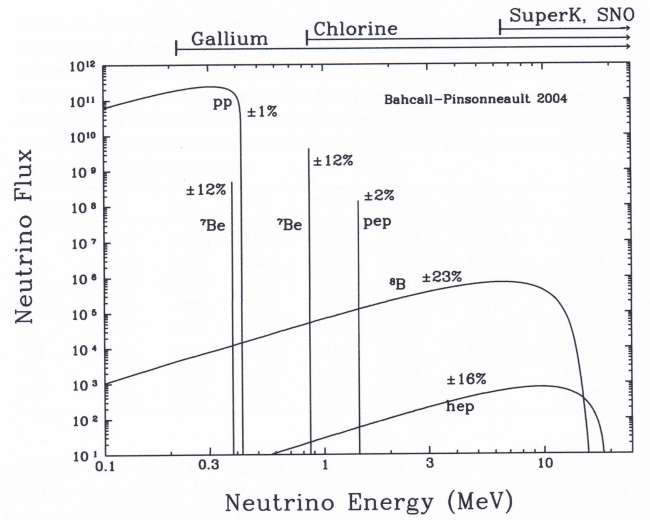
\includegraphics[width=\textwidth,height=(\textheight-11mm),keepaspectratio]{nuspectrum}
\caption{Spettro dei neutrini solari e sensibilit\'a strumenti di rivelazione.}
\end{figure}

Risultati.

\begin{align*}
\Phi^{(CC)}\approx1.76*10^6\frac{\Pnue}{cm^2*s}\\
\Phi^{(CN)}\approx5.09*10^6\frac{\nu_x}{cm^2*s}
\end{align*}

\subsection{Soluzione problema neutrini}
I neutrini cambiano flavour nel tragitto Sole-Terra.

\end{document}